\newpage
\section{Decisions}

\vspace{5mm}
\begin{center}
    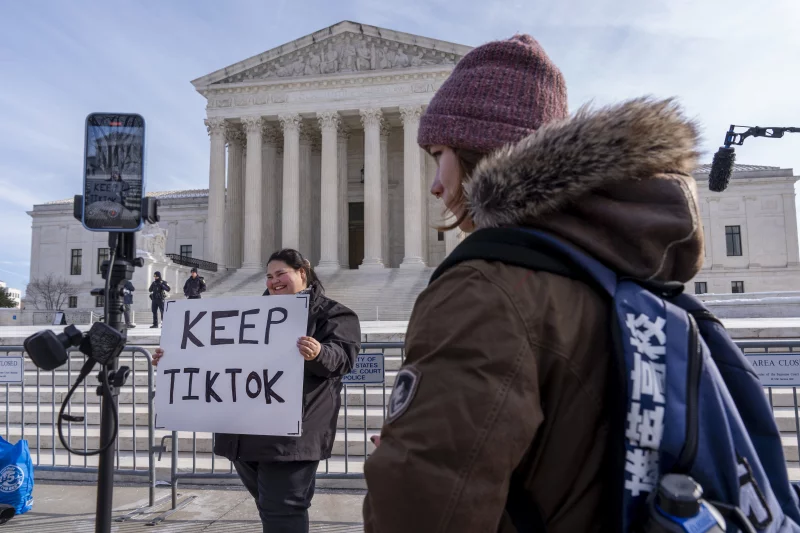
\includegraphics[width=350px]{images/decisions_introduction.png}\\[2mm]
    \footnotesize{Photo Credit: AP/Jacquelyn Martin}
\end{center}

\vspace{5mm}

\begin{center}
\begin{table}[H]
    \normalsize
    \centering
    \caption{What's Included (Decisions)}
    \label{tab:decisions_intro}
    \vspace{1mm}
    \begin{tabularx}{\textwidth}{>{\centering\arraybackslash}p{0.2\textwidth}>{\centering\arraybackslash}p{0.2\textwidth}>{\centering\arraybackslash}X}
        \toprule
        Area & Topic & Description \\
        \midrule
        Overview & Case Information & \RaggedRight Overview of cases decided by the Court, including: Dates of Argument and Decision, Majority Author and Majority/Minority Coalition Sizes, etc. \\
        \addlinespace
        & Vote Matrices & \RaggedRight Justice-level voting behaviors by case and Justice. \\
        \addlinespace
        & Vote Alignments & \RaggedRight Proportion of shared voting preferences by Justice-level pairing. \\
        \addlinespace
        Opinions & Opinion Authorship & \RaggedRight Term-level summary of Justice-level opinion authorship behaviors.  \\
        \addlinespace
        Historical Comparisons & Coalition Sizes & \RaggedRight Comparison to previous terms' rates of varying coalition sizes. \\
        \addlinespace
        & Unanimity & \RaggedRight Comparison to previous terms' rates of unanimity. \\

        \bottomrule
    \end{tabularx}
\end{table}
\end{center}

\newpage

\begin{center}
\vspace{5mm}
\Huge\textbf{\subsection{\underline{Note on Decision Coding}}}
\end{center}

\noindent We recognize that the array of potential case-level votes do not always neatly align with a definitive indicator that a Justice should be considered a member of the Majority or Minority (\emph{Dissenting}) coalition. In particular, votes by Justices \emph{Concurring and Dissenting In Part}, \emph{Concurring in Judgement}, joining (and/or authoring) several concurrences, etc., are not as clear of an indicator as authoring or simply joining the majority. These special votes could lead to varying records of majority and minority coalitions sizes depending on the source. For example, a decision rendered with a single Justice authoring an opinion \emph{Concurring In Part, and Dissenting in Part} could reasonbly be coded as either (9-0) or (8-1), given that the Justice neither fully joined -- nor fully dissented -- from the Court's majority opinion. \\

To maintain methodological consistency, we code choices to join the \textbf{Minority} (\emph{Dissent}) as instances where a Justice (1) Authored a Dissenting Opinion or (2) \textbf{Only} Joined a Dissenting Opinion. Below we list the cases impacted by this coding scheme. \\

\begin{itemize}

\item \emph{Trump v. J.G.G} (24A931) -- Decided January 22, 2025


\end{itemize}

\begin{center}
\vspace{5mm}
\Huge\textbf{\subsection{\underline{Additional Notes: Opinion Consolidations}}}
\end{center}

\begin{itemize}

%\item Given the post-argument consolidation of \emph{Loper Bright Enterprises v. Raimondo} (22-451) with \emph{Relentless, Inc., et al. v. Department of Commerce} (22-1219), we report the outcome collectively under \emph{Loper Bright} as (6-3) with Justice Jackson joining Justice Sotomayor's dissent (though Justice Jackson did not participate in the proceedings of 22-451).
\item

\end{itemize}
